%!TEX root = paper.tex
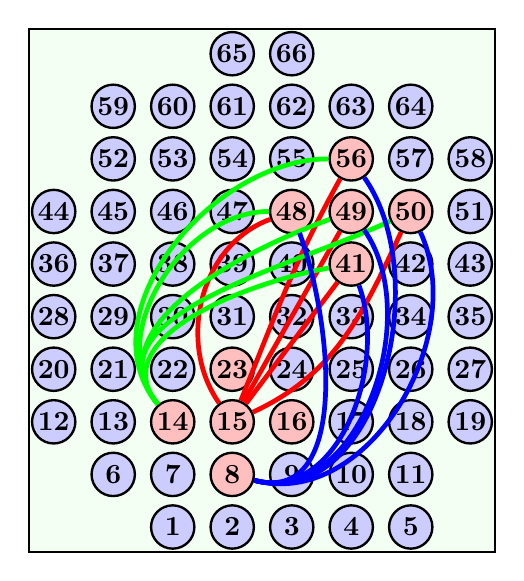
\begin{tikzpicture}[-,red, line width=0.06cm,font=\bfseries,draw=black] 
	\tikzstyle{every node}=[circle,ultra thick,draw=black,fill=white,text=black,minimum size=0.55cm,line width=0.03cm,inner sep=0.8pt]
	\tikzstyle{HC} =[fill=blue!20] % HC = healthy control node
	\tikzstyle{DS} =[fill=red!25]  % DS = disease node
	\matrix [rectangle,row sep=2.5pt, column sep=5pt,draw=black,fill=green!5,line width=0.025cm] % 
	{
				    ;&				;&				 ;& \node(65)[HC]{65} ;& \node(66)[HC]{66} ;\\
		 		    ;& \node(59)[HC]{59} ;& \node(60)[HC]{60} ;& \node(61)[HC]{61} ;& \node(62)[HC]{62} ;& \node(63)[HC]{63} ;& \node(64)[HC]{64} ;& ;\\
		 		    ;& \node(52)[HC]{52} ;& \node(53)[HC]{53} ;& \node(54)[HC]{54} ;& \node(55)[HC]{55} ;& \node(56)[DS]{56} ;& \node(57)[HC]{57} ;& \node(58)[HC]{58} ;\\
	 \node(44)[HC]{44} ;& \node(45)[HC]{45} ;& \node(46)[HC]{46} ;& \node(47)[HC]{47} ;& \node(48)[DS]{48} ;& \node(49)[DS]{49} ;& \node(50)[DS]{50} ;& \node(51)[HC]{51} ;\\
	 \node(36)[HC]{36} ;& \node(37)[HC]{37} ;& \node(38)[HC]{38} ;& \node(39)[HC]{39} ;& \node(40)[HC]{40} ;& \node(41)[DS]{41} ;& \node(42)[HC]{42} ;& \node(43)[HC]{43} ;\\
	 \node(28)[HC]{28} ;& \node(29)[HC]{29} ;& \node(30)[HC]{30} ;& \node(31)[HC]{31} ;& \node(32)[HC]{32} ;& \node(33)[HC]{33} ;& \node(34)[HC]{34} ;& \node(35)[HC]{35} ;\\
	 \node(20)[HC]{20} ;& \node(21)[HC]{21} ;& \node(22)[HC]{22} ;& \node(23)[DS]{23} ;& \node(24)[HC]{24} ;& \node(25)[HC]{25} ;& \node(26)[HC]{26} ;& \node(27)[HC]{27} ;\\
	 \node(12)[HC]{12} ;& \node(13)[HC]{13} ;& \node(14)[DS]{14} ;& \node(15)[DS]{15} ;& \node(16)[DS]{16} ;& \node(17)[HC]{17} ;& \node(18)[HC]{18} ;& \node(19)[HC]{19} ;\\
		 		    ;& \node(6)[HC]{6} 	;& \node(7)[HC]{7} 	 ;& \node(8)[DS]{8}	  ;& \node(9)[HC]{9}   ;& \node(10)[HC]{10} ;& \node(11)[HC]{11} ;&  ;\\
	 			    ;&				;& \node(1)[HC]{1} 	 ;& \node(2)[HC]{2}	  ;& \node(3)[HC]{3}   ;& \node(4)[HC]{4}   ;& \node(1)[HC]{5}   ;&  ;\\
	};
	% edge group red
	\tikzstyle{col}=[red] 
	\draw(15)to[](41)[col];
	\draw(15)to[out=125,in=-160](48)[col];
	\draw(15)to[](49)[col];
	\draw(15)to[out=25,in=-115](50)[col];
	\draw(15)to[out=68,in=-119](56)[col];
	% edge group green
	\tikzstyle{col}=[green!100] 
	\draw(14)to[out=130,in=190](41)[col];
	\draw(14)to[out=130,in=180](48)[col];
	\draw(14)to[out=130,in=200](49)[col];
	\draw(14)to[out=130,in=205](50)[col];
	\draw(14)to[out=130,in=180](56)[col];	
	% edge group blue
	\tikzstyle{col}=[blue] 
	\draw(8)to[out=-15,in=-70](41)[col];
	\draw(8)to[out=-15,in=-70](48)[col];
	\draw(8)to[out=-15,in=-55](49)[col];
	\draw(8)to[out=-15,in=-65](50)[col];
	\draw(8)to[out=-15,in=-55](56)[col];
\end{tikzpicture}
\begin{tikzpicture}[-,red, line width=0.06cm,font=\bfseries,draw=black] 
	\tikzstyle{every node}=[circle,ultra thick,draw=black,fill=white,text=black,minimum size=0.55cm,line width=0.03cm,inner sep=0.8pt]
	\tikzstyle{HC} =[fill=blue!20] % HC = healthy control node
	\tikzstyle{DS} =[fill=red!25]  % DS = disease node
	\matrix [rectangle,row sep=2.5pt, column sep=5pt,draw=black,fill=green!5,line width=0.025cm] % 
	{
				    ;&				;&				 ;& \node(65)[HC]{65} ;& \node(66)[HC]{66} ;\\
		 		    ;& \node(59)[HC]{59} ;& \node(60)[HC]{60} ;& \node(61)[HC]{61} ;& \node(62)[HC]{62} ;& \node(63)[HC]{63} ;& \node(64)[HC]{64} ;& ;\\
		 		    ;& \node(52)[HC]{52} ;& \node(53)[HC]{53} ;& \node(54)[HC]{54} ;& \node(55)[HC]{55} ;& \node(56)[DS]{56} ;& \node(57)[HC]{57} ;& \node(58)[HC]{58} ;\\
	 \node(44)[HC]{44} ;& \node(45)[HC]{45} ;& \node(46)[HC]{46} ;& \node(47)[HC]{47} ;& \node(48)[DS]{48} ;& \node(49)[DS]{49} ;& \node(50)[DS]{50} ;& \node(51)[HC]{51} ;\\
	 \node(36)[HC]{36} ;& \node(37)[HC]{37} ;& \node(38)[HC]{38} ;& \node(39)[HC]{39} ;& \node(40)[HC]{40} ;& \node(41)[DS]{41} ;& \node(42)[HC]{42} ;& \node(43)[HC]{43} ;\\
	 \node(28)[HC]{28} ;& \node(29)[HC]{29} ;& \node(30)[HC]{30} ;& \node(31)[HC]{31} ;& \node(32)[HC]{32} ;& \node(33)[HC]{33} ;& \node(34)[HC]{34} ;& \node(35)[HC]{35} ;\\
	 \node(20)[HC]{20} ;& \node(21)[HC]{21} ;& \node(22)[HC]{22} ;& \node(23)[DS]{23} ;& \node(24)[HC]{24} ;& \node(25)[HC]{25} ;& \node(26)[HC]{26} ;& \node(27)[HC]{27} ;\\
	 \node(12)[HC]{12} ;& \node(13)[HC]{13} ;& \node(14)[DS]{14} ;& \node(15)[DS]{15} ;& \node(16)[DS]{16} ;& \node(17)[HC]{17} ;& \node(18)[HC]{18} ;& \node(19)[HC]{19} ;\\
		 		    ;& \node(6)[HC]{6} 	;& \node(7)[HC]{7} 	 ;& \node(8)[DS]{8}	  ;& \node(9)[HC]{9}   ;& \node(10)[HC]{10} ;& \node(11)[HC]{11} ;&  ;\\
	 			    ;&				;& \node(1)[HC]{1} 	 ;& \node(2)[HC]{2}	  ;& \node(3)[HC]{3}   ;& \node(4)[HC]{4}   ;& \node(1)[HC]{5}   ;&  ;\\
	};
	%********************** Style 2 **************************%
%	% edge group red
	\tikzstyle{col}=[black] 
	\draw(23)to[out=15,in=-90](41)[col];
	\draw(23)to[](48)[col];
	\draw(23)to[](49)[col];
	\draw(23)to[out=0,in=-90](50)[col];
	\draw(23)to[out=90,in=180](56)[col];

	% edge group yellow
	\tikzstyle{col}=[myorange] 
	\draw(16)to[in=-80](41)[col];
	\draw(16)to[](48)[col];
	\draw(16)to[out=78,in=-120](49)[col];
	\draw(16)to[out=30,in=-80](50)[col];
	\draw(16)to[out=82,in=-123](56)[col];
\end{tikzpicture}
